\newpage\section{Aufgabe 4}
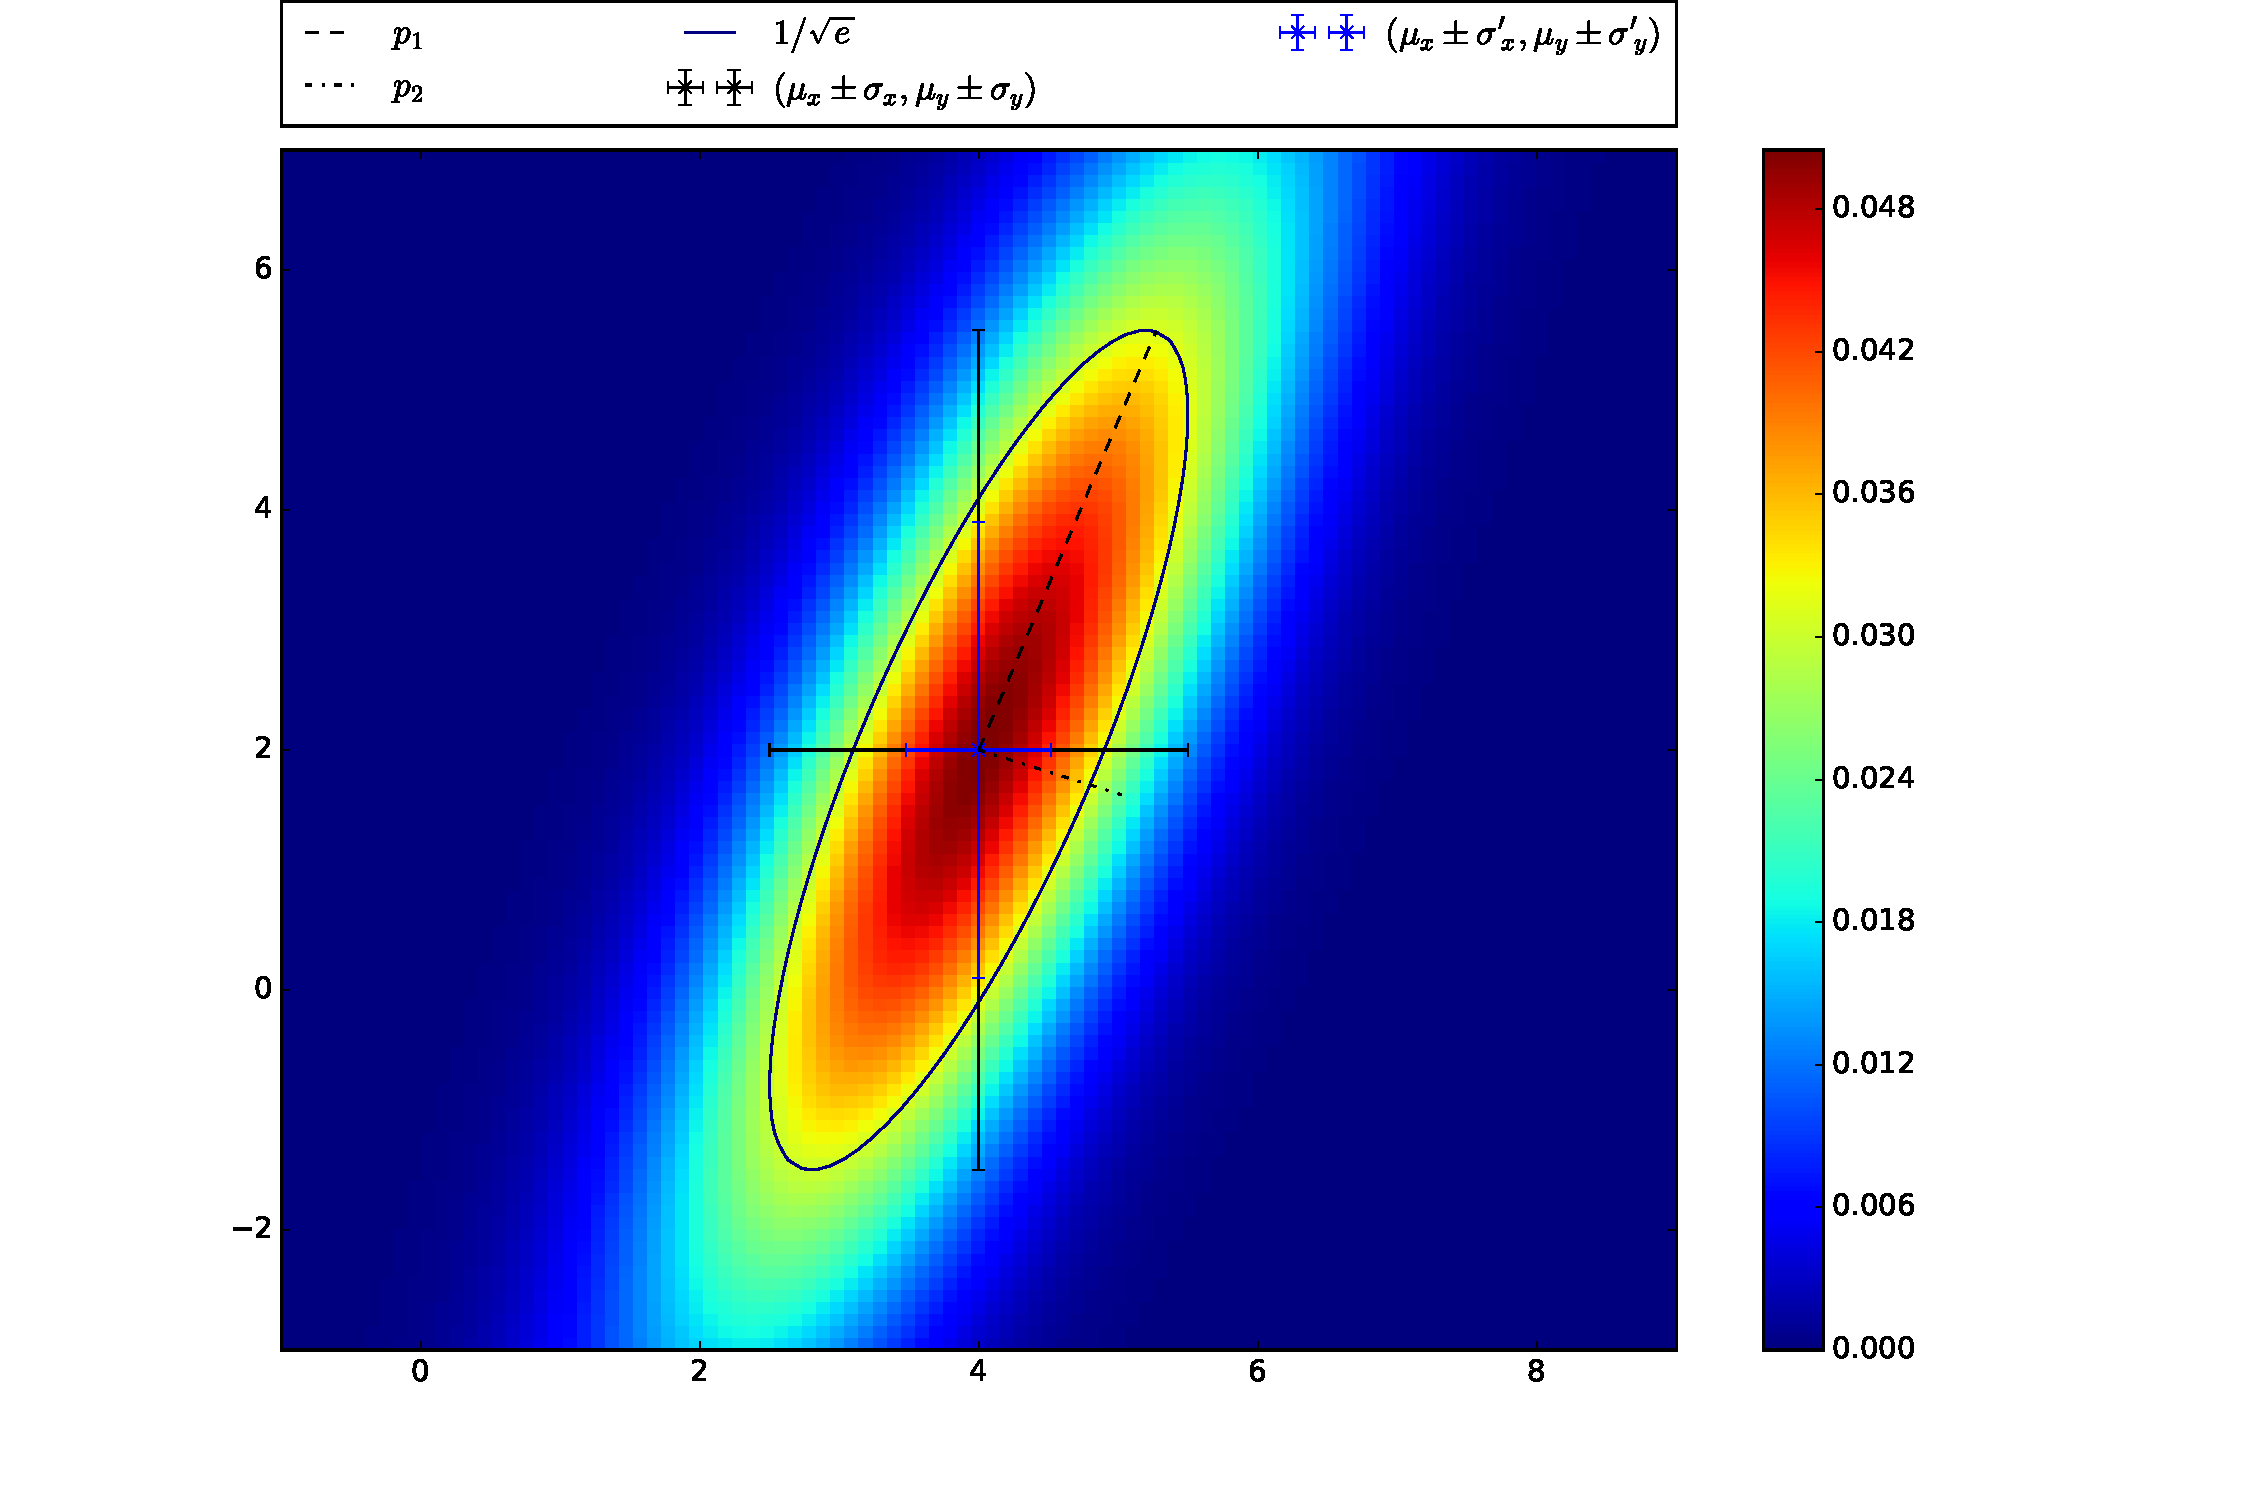
\includegraphics[width=\textwidth]{aufg4.pdf}
\subsection{a)}
\begin{equation*}
\rho = \frac{cov(x,y)}{\sigma_x\sigma_y} = \SI{0.8}{}
\end{equation*}
\subsection{b)}
\begin{align*}
f(x,y) = k \cdot \exp \Biggl(\frac{-0.5}{1-\rho^2}\Biggl(\biggl(\frac{x-\mu_x}{\sigma_x}\biggr)^2-2\rho\frac{x-\mu_x}{\sigma_x}\frac{y-\mu_y}{\sigma_y}+\biggl(\frac{x-\mu_x}{\sigma_x}\biggr)^2\Biggr)\Biggr)\\
\Rightarrow f_\text{max}=f(\mu_x,\mu_y)=k\\
\\
\Rightarrow f(x,y)=\frac{f_\text{max}}{\sqrt{\text{e}}}=\frac{k}{\sqrt{\text{e}}}\\
\\
\Rightarrow \frac{1}{1-\rho^2}\Biggl(\biggl(\frac{x-\mu_x}{\sigma_x}\biggr)^2-2\rho\frac{x-\mu_x}{\sigma_x}\frac{y-\mu_y}{\sigma_y}+\biggl(\frac{x-\mu_x}{\sigma_x}\biggr)^2\Biggr) = 1
\end{align*}
Eine Ellipsengleichung.
\subsection{c)}
\begin{equation*}
\begin{pmatrix}
1/{\sigma'_x}^2 & 0\\0 & 1/{\sigma'_y}^2
\end{pmatrix}= M^{-1} B M
\end{equation*}
\begin{equation*}
B = \frac{1}{{\sigma_x}^2{\sigma_y}^2-\text{cov}^2(x,y)}\begin{pmatrix}
\sigma{\sigma_y}^2 & -\text{cov}(x,y)\\-\text{cov}(x,y) & {\sigma_x}^2\end{pmatrix} = \begin{pmatrix} 0.22675737 & -0.42 \\-0.42 &  1.2345679\end{pmatrix}
\end{equation*}
\begin{equation*}
M =  \begin{pmatrix}-0.342268 & -0.939602\\0.939602 &-0.342268\end{pmatrix}
\end{equation*}
\begin{align*}
\sigma'_x = \SI{ 0.518496228435}{}\\
\sigma'_y = \SI{ 1.898865186}{}
\end{align*}
\subsection{d)}
\begin{equation*}
\alpha = 0.5\arctan(2\rho\sigma_x\sigma_y/(\sigma_x^ 2-\sigma_y^ 2)) = \SI{20.0151296359}{\deg}
\end{equation*}
\begin{align*}
p_1 = \sqrt{((1-\rho^2)/(\cos(\alpha)^2/\sigma_x^2-2*\rho\sin(\alpha)\cos(\alpha)/\sigma_x/\sigma_y+\sin(\alpha)^2/\sigma_y^2))} = \SI{3.71213295653}{}\\
p_2 = \sqrt{((1-\rho^2)/(\sin(\alpha)^2/\sigma_x^2-2*\rho\sin(\alpha)\cos(\alpha)/\sigma_x/\sigma_y+\cos(\alpha)^2/\sigma_y^2))} = \SI{1.08833663572}{}
\end{align*}
